%%% Dateikodierung: UTF-8
%%% äöüÄÖÜß  <-- keine deutschen Umlaute hier? UTF-faehigen Editor verwenden!

%%% Magic Comments zum Setzen der korrekten Parameter in kompatiblen IDEs
% !TeX encoding = utf8
% !TeX program = pdflatex 
% !TeX spellcheck = de_DE
% !BIB program = biber

\documentclass[bachelor,german,smartquotes]{hgbthesis}

% Zulässige Optionen in [..]: 
%    Typ der Arbeit: 'diploma', 'master' (default), 'bachelor', 'internship' 
%    Hauptsprache: 'german' (default), 'english'
%    Option zur Umwandlung in typografische Anführungszeichen: 'smartquotes'
%    APA Zitierstil: 'apa'
%%%-----------------------------------------------------------------------------

\RequirePackage[utf8]{inputenc} % bei Verw. von lualatex oder xelatex entfernen!

\graphicspath{{images/}}  % Verzeichnis mit Bildern und Grafiken
\logofile{logo}           % Logo-Datei: images/logo.pdf (kein Logo: \logofile{})
\bibliography{references} % Biblatex-Literaturdatei (references.bib)
%%%-----------------------------------------------------------------------------
% Angaben für die Titelei (Titelseite, Erklärung etc.)
%%%-----------------------------------------------------------------------------

\title{Erkennung und Klassifikation von Wildtieren mittels Computer Vision}
\author{Lukas Nikolaus Nepelius}
\programname{Medizin- und Bioinformatik}

%\programtype{Fachhochschul-Bachelorstudiengang} % auswählen/editieren
\programtype{Fachhochschul-Bachelorstudiengang}

\placeofstudy{Hagenberg}
\dateofsubmission{2021}{07}{15} % {YYYY}{MM}{DD}

\advisor{DI (FH) Dr. Gerald Zwettler MSc} % optional

%\strictlicense % restriktive Lizenz anstatt Creative Commons (nicht empfohlen!)

%%%-----------------------------------------------------------------------------
\begin{document}
%%%-----------------------------------------------------------------------------

%%%-----------------------------------------------------------------------------
\frontmatter                                       % Titelei (röm. Seitenzahlen)
%%%-----------------------------------------------------------------------------

\maketitle
\tableofcontents

\chapter{Vorwort}

 % Ein Vorwort ist optional
\chapter{Kurzfassung}



\chapter{Abstract}


\begin{english} %switch to English language rules
This should be a 1-page (maximum) summary of your work in English.
%und hier geht dann das Abstract weiter...
\end{english}

			

%%%-----------------------------------------------------------------------------
\mainmatter                             % Hauptteil (ab hier arab. Seitenzahlen)
%%%-----------------------------------------------------------------------------

\chapter{Einleitung}
\label{cha:Einleitung}


\chapter{Grundlagen}
\label{cha:Grundlagen}

\section{OpenCV Grundlagen}
OpenCV ist eine umfangreiche Bibliothek für Bildverarbeitungs- und Computer Vision Methoden \cite{IntroToOpenCV} \cite{OpenCVPython}. Die Benützung von OpenCV bringt einige Vorteile, die durch die grundsätzliche Architektur des Frameworks ermöglicht werden. Ein Aspekt wäre das Speichermanagement Konzept, das das Lesen / Schreiben von Bildern und Videos in OpenCV, ohne Speicher manuell allokieren oder wieder freigeben zu müssen, ermöglicht.\par
Die Bibliothek wurde erstmals Ende der 1990er Jahre von der Firma Intel als Forschungsprojekt in Auftrag gegeben. Die Vision hinter dem Projekt war, auf Computer Vision aufbauende Algorithmen frei verfügbar und optimiert zu implementieren, damit das Neuerfinden von schon etablierten Algorithmen reduziert und die Forschung in diesem Bereich vorangetrieben wird. Entwickler sollen auf den Methoden des Frameworks aufbauen und somit den Programmcode leichter verständlich machen. Die erste Version von OpenCV wurde im Jahr 2000 auf der IEEE Conference on Computer Vision and Pattern Recognition präsentiert und seither kontinuierlich weiterentwickelt.\par
OpenCV umfasst eine Menge an Methoden mit denen man Bild- und Videodaten in jeglicher Art und Weise manipulieren kann. Dazu zählen Verfahren der Bildbearbeitung und Bildverarbeitung wie Kontrastanhebung, Kantendetektion, Optical Flow oder auch komplexere Methoden der Computer Vision wie Objekterkennung, Klassifierung mittels Machine Learning. Aufgeteilt ist das Framework in verschiedene Module, die dann unter Anderem Funktionen für die Bildmanipulation enthalten. Das wichtigste Modul in OpenCV heißt Core und ist für die grundlegenden Datentypen, Datenstrukturen und die Speicherzuweisung zuständig. Eines dieser wichtigen Datentypen ist \textit{Mat}, das im Prinzip ein Bild in Matrizenform abspeichert. Ein Überblick der wichtigsten Module in OpenCV ist in \autoref{tab:table_cv} zu sehen.
\newpage
\begin{table}[]
    \centering
    \begin{tabular}[h]{|l||l|}
        \hline
        \textbf{Highgui} & GUI von OpenCV \\[2.5pt]
        \textbf{Video} & Bewegungsanalysen und Objektverfolgung \\[2.5pt]
        \textbf{Features2d} & Features herausfiltern, beschreiben und verbinden \\[2.5pt]
        \textbf{Imgcodecs} & Bilder lesen und schreiben \\[2.5pt]
        \textbf{videoio} & Videos lesen und schreiben \\[2.5pt]
        \textbf{dnn} & Objekterkennung und Klassifizierung mittels Deep Learning \\ \hline
    \end{tabular}
    \caption{Überblick der wichtigsten Module in OpenCV}
    \label{tab:table_cv}
\end{table}

\section{YOLO}

Folgendes Kapitel wurde aus dem wissenschaftlichen Artikel über den YOLO Algorithmus von den Entwickelern von YOLO zusammengefasst \cite{YOLOOfficialPub}.

Bei dem YOLO (You only look once) Algorithmus wird ein einzelnes neuronales Netzwerk verwendet, dass die Bounding Boxen der Objekte auf Bildern voraussagt. Der YOLO Algorithmus ist im Vergleich zu anderen State-Of-The-Art Methoden wie dem RCNN (Recurrent Convolutional Neural Network) relativ schnell. Er verarbeitet im Schnitt 45 Bilder in der Sekunde, die abgespeckte Version des Algorithmuses schafft sogar 155 Bilder pro Sekunde. In Kontrast zu RCNN benötigt YOLO nur einen Prozess, der alle Objekte auf dem gegebenen Bild erkennt und klassifiziert, woher auch das Akronym "You only look once" abgeleitet ist.
\begin{figure}[h]
    \centering
    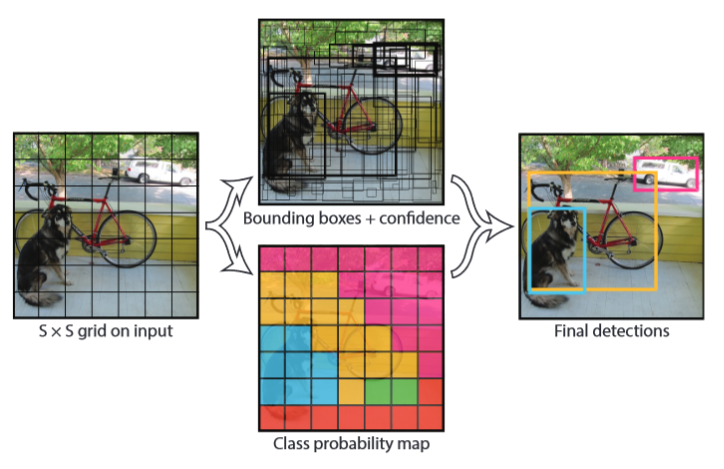
\includegraphics{images/YOLO_func.PNG}
    \caption{Überblick der wichtigsten Funktionsweisen des YOLO Algorithmuses.}
\end{figure}
\newpage
Der Algorithmus funktioniert so, dass zuerst alle Eingabebilder in eine S x S große Matrix von Zellen aufgeteilt werden. Die Bilder werden auch so skaliert, dass sie alle die gleiche Größe haben. Dabei bestimmt jede Zelle in der Matrix die Bounding Boxen und eine prozentuale Konfidenz. Diese Konfidenz gibt an wie sicher sich der Algorithmus ist, dass sich in der aktuellen Zelle ein Objekt befindet. Ist der Konfidenz-Wert gleich Null, dann befindet sich an dieser Stelle kein Objekt, befindet sich aber ein Objekt in der Zelle so wird das Intersection Over Union (IOU) von der vorhergesagten und der tatsächlichen Bounding Box des Objektes gebildet. Zusätzlich wird für jede Zelle auch noch die Wahrscheinlichkeit für die jeweiligen Klassen gespeicher. Diese Wahrscheinlichkeit gibt an, wie sicher sich der Algorithmus ist, dass es sich bei gegebenem Objekt um eine konkrete Klasse handelt. Beide dieser Wahrscheinlichkeiten werden dann multipliziert, sodass ein Wert entsteht, der darüber Aussage gibt wie gut eine Klasse zu einer Bounding Box bzw. wie gut eine Bounding Box zu einem Objekt passt.\par
\begin{figure}[h]
    \centering
    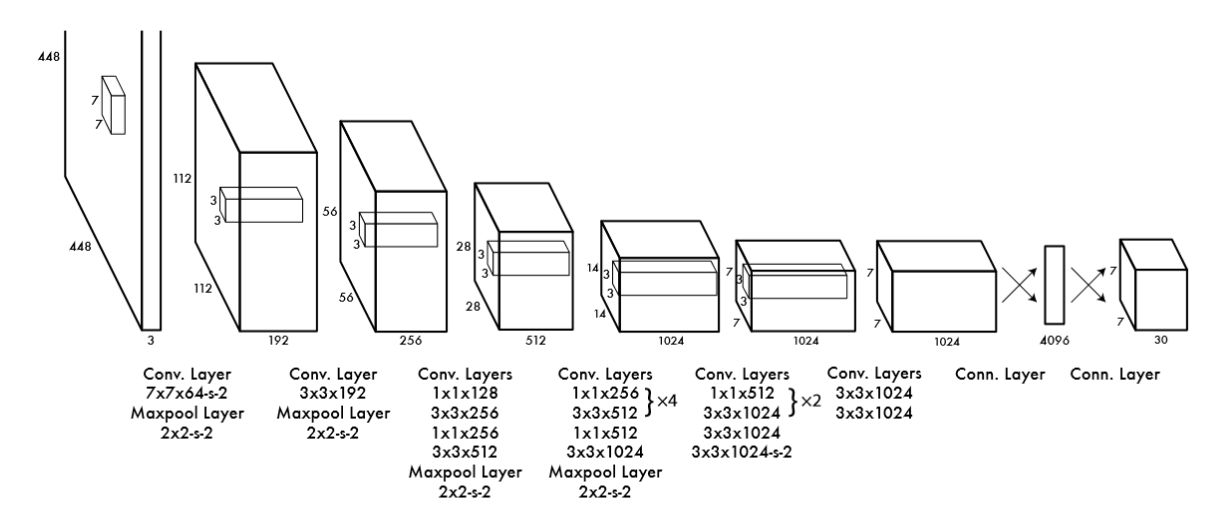
\includegraphics[width=\linewidth]{images/YOLO_network.PNG}
    \caption{Die Abbildung skizziert den Aufbau und die Struktur des CNN.}
    \label{fig:my_label}
\end{figure}
Beim Convolutional Neural Network von YOLO ist der erste Layer, der sogenannte Input Layer, für die Bestimmung der Features im Bild zuständig. Die Fully Connected Schichten im Hidden Layers Bereich des Netzwerks werden die Wahrscheinlichkeiten und Koordinaten der Bounding Boxen der Objekte berechnet. In der standard Version von YOLO gibt es im Netzwerk 24 Convolutional und 2 Fully Connected Layers. Das Netzwerk der "tiny" Version von YOLO besitzt nur 9 statt 24 Convolutional Layers.\par
Trainiert wird das CNN mit dem ImageNet [cite] Datensatz, das Bilder der Größe 448 x 448 pixel entgegennimmt. Die Höhe, Breite, x- und y-Koordinaten der Bounding Boxen werden relativ zur Bildgröße normalisiert, sodass jeweils ein Wert zwischen 0 und 1 verwendet wird.\par
Die sogenannte Non-Maximum Suppression Methode kann dem Algorithmus ergänzt werden, um ineinander verschachtelte Boxen am gleichen Objekt zu verhindern/reduzieren.\par
Jede Zelle der Matrix kann nur maximal 2 Boxen und eine Klasse vorhersagen. Der YOLO Algorithmus hat Probleme mit kleinen und gruppierten Objekten, wie zum Beispiel einem Vogelschwarm. Die meisten Fehler unter YOLO passieren mit falschen Lokalisationen von Bounding Boxen.\par
Der große Vorteil, den YOLO gegenüber RCNN und ähnlichen Methoden hat, ist, dass er nur ein Convolutional Neural Network benötigt, der die ganze Arbeit der Objekterkennung und Klassifikation erledigt.

\section{Objektverfolgung (Object Tracking)}
Eines der Probleme beim reinen Erkennen von Objekten ist, dass der Algorithmus Bilder in einem Video isoliert betrachtet und analysiert. Ein Zählen der Objekte ist daher nicht möglich, was aber durchaus sinnvoll zum Erheben von relevanten Daten der Tiere wäre. Um nun diesen Zusammenhang zwischen den Bildern und den Objekten herzustellen, müssen die Objekte sozusagen verfolgt werden. In anderen Worten muss der Algorithmus das selbe Objekt über mehrere Bilder hinweg bestimmen. Aus diesem Grund werden nun Algorithmen zur Objektverfolgung besprochen.\par
Die frei verfügbare Bibliothek OpenCV stellt mehrere state-of-the-art Verfahren diesbezüglich zur Verfügung unter anderem die CSRT Methode, die nach dem Schema des Discriminative Correlation Filter with Channel and Spatial Reliability (CSR-DCF) Verfahrens implementiert wurde. In weiterer Folge habe ich mich für dieses Verfahren entschieden aufgrund der hohen Präzision der Methode. Die Videos vom Nationalpark Hohe Tauern haben eine relativ geringe Auflösung und Bildwiederholrate, weshalb mir dieser Aspekt sehr wichtig ist und ich die Performanzeinbußen der Methode tolerierbar sind. Im folgenden Absatz wird die Methode des CSR-DCF \cite{ObjectTrackingCSRDCF} bechrieben.\par
Der CSRT Tracker von OpenCV funktioniert mittels Discriminative Correlation Filter (DCF) in Kombination mit Channel and Spatial Reliability. Bei DCF Methoden wird das Bild in den Frequenzraum mit der Fast Fourrier Transformation (FFT) überführt. Der Nachteil bei dieser Transformation ist, dass dabei unnatürliche kreisförmige Strukturen entstehen, die den Suchbereich des Bildes verzerren. Das zweite Problem bei DCF Methoden ist, dass der Algorithmus annimmt, dass die Box um das Objekt nach der x- bzw. y-Achse ausgerichtet wird. Dadurch können unregelmäßig geformte Objekte oder auch hohle Objekte nicht erkannt werden.\par
Diese zwei Probleme werden mit dem CSR-DCF gelöst indem eine sogenannte Spatial Reliability Map erzeugt wird. Bei diesem Verfahren wird ein Trainingsbereich mit einer Box festgelegt, dann wird die A-Priori-Wahrscheinlichkeit durch ein Markow-Netzwerk berechnet, die Wahrscheinlichkeit des Objektes bezüglich Vorder- und Hintergrund Farbmodellen und die A-posteriori-Wahrscheinlichkeit nach Markov-Zufallsfeld Regulierung bestimmt. Am Schluss wird noch der Trainingsbereich mit der finalen binären Reliability Map maskiert.
\newpage
\begin{figure}[h]
    \centering
    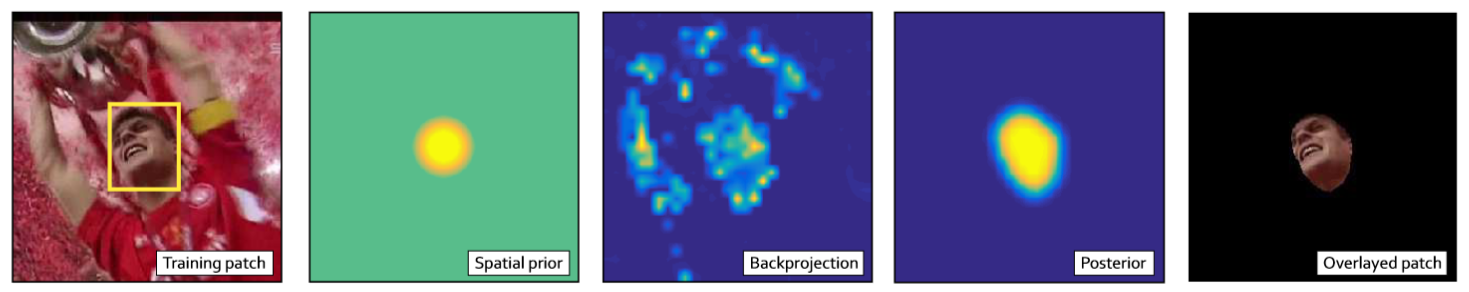
\includegraphics[width=\linewidth]{images/CSR_DCF_Pipeline.png}
    \caption{Einzelne Schritte beim Erzeugen einer Spatial Reliability Map.}
\end{figure}

Im Prinzip geht der Algorithmus in zwei Schritten vor: Zuerst wird in einem Lokalisationsschritt die neue Zielposition des Objektes berechnet. Anhand dieser Position wird dann anschließend die Größe geschätzt. Der zweite Schritt ist ein Aktualisierungsvorgang, bei dem jeweils für Vorder- und Hintergrund ein Histogramm erstellt, die Reliability Map berechnet, ein neuer Filter geschätzt und die Channel Reliability erzeugt wird.

\begin{figure}[h]
    \centering
    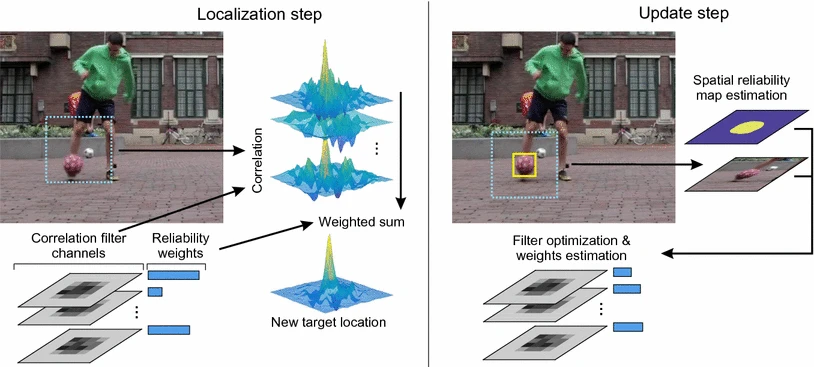
\includegraphics{images/CSR_DCF_Localisation_Update.png}
    \caption{https://link.springer.com/article/10.1007/s11263-017-1061-3/figures/6. Der Lokalisationsschritt wird initial durchgeführt um die umgebende Box des Objektes festzustellen. Pro Bild wird dann die Spatial Reliability Map berechnet und der Filter optimiert.}
\end{figure}

Der eben beschrieben Algorithmus arbeitet mit HOG und Colornames \cite{ColornamesFeatures} Features, was ein präziseres Tracking-Ergebnis ermöglicht. Vergleicht man die CSR-DCF Methode mit anderen state-of-the-art Ansätzen wie dem SRDCF \cite{ObjectTrackingSRDCF} oder dem CFLB \cite{ObjectTrackingCFLB} vor allem in Hinsicht auf Präzision, dann schneidet die CSR-DCF Methode vergleichsweise gut ab. Objektverfolgungsverfahren wie der KCF sind zwar performanter, andererseits leidet aber auch die Qualität des Tracking-Ergebnisses darunter.\par
Zusammenfassend führt der CSR-DCF Ansatz mit dem Erstellen einer Reliabilty Map und dem Adaptieren des Filters, zu einem genaueren Verfolgen des Objektes. Man umgeht dabei auch die zwei Probleme des DCF Verfahrens, einerseits die kreisförmigen Verzerrungen durch die Fourrier Transformation und dem Rechteck-Problem. 

%%%-----------------------------------------------------------------------------
\appendix                                                               % Anhang 
%%%-----------------------------------------------------------------------------

% Anhänge

%%%-----------------------------------------------------------------------------
\backmatter                          % Schlussteil (Quellenverzeichnis und dgl.)
%%%-----------------------------------------------------------------------------

\MakeBibliography % Quellenverzeichnis

%%%-----------------------------------------------------------------------------
% Messbox zur Druckkontrolle
%%%-----------------------------------------------------------------------------

\chapter*{Messbox zur Druckkontrolle}



\begin{center}
{\Large --- Druckgröße kontrollieren! ---}

\bigskip

\calibrationbox{100}{50} % Angabe der Breite/Hoehe in mm

\bigskip

{\Large --- Diese Seite nach dem Druck entfernen! ---}

\end{center}



%%%-----------------------------------------------------------------------------
\end{document}
%%%-----------------------------------------------------------------------------
